\documentclass{standalone}
\usepackage{tikz}
\usetikzlibrary{patterns, positioning}


\begin{document}
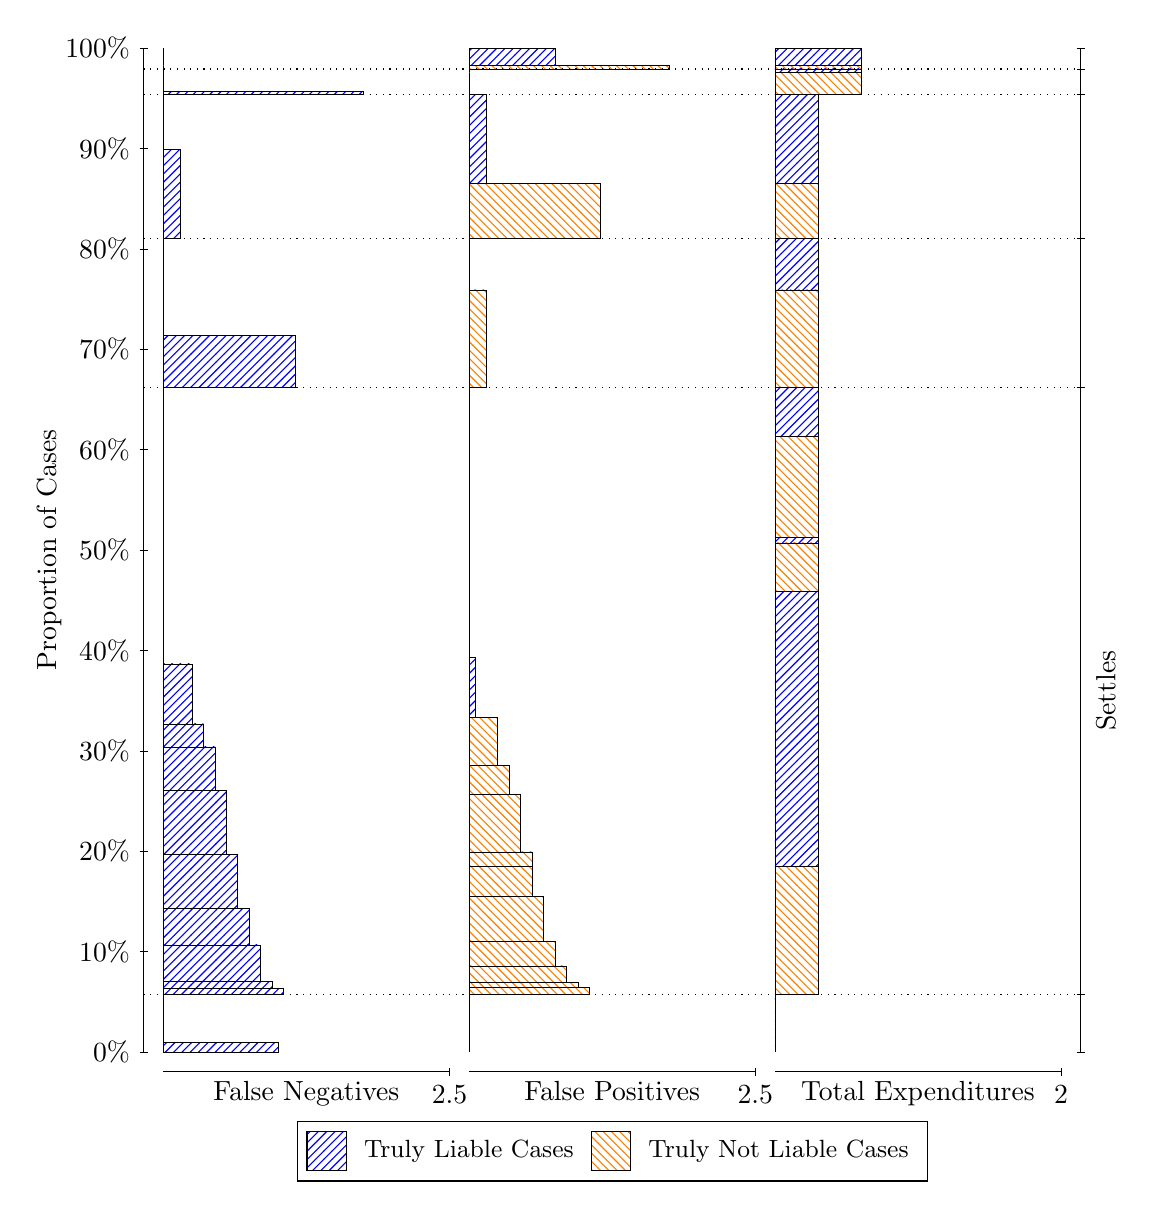
\begin{tikzpicture}
\draw[black, very thin] (1.5,1.75) -- (1.5,14.5);
\node[rotate=90, text=black, anchor=center] at (0.3, 8.125) {Proportion of Cases};
\draw[black, very thin] (1.45,1.75) -- (1.55,1.75);
\node[text=black, anchor=east] at (1.45, 1.75) {0\%};
\draw[black, very thin] (1.45,3.025) -- (1.55,3.025);
\node[text=black, anchor=east] at (1.45, 3.025) {10\%};
\draw[black, very thin] (1.45,4.3) -- (1.55,4.3);
\node[text=black, anchor=east] at (1.45, 4.3) {20\%};
\draw[black, very thin] (1.45,5.575) -- (1.55,5.575);
\node[text=black, anchor=east] at (1.45, 5.575) {30\%};
\draw[black, very thin] (1.45,6.85) -- (1.55,6.85);
\node[text=black, anchor=east] at (1.45, 6.85) {40\%};
\draw[black, very thin] (1.45,8.125) -- (1.55,8.125);
\node[text=black, anchor=east] at (1.45, 8.125) {50\%};
\draw[black, very thin] (1.45,9.4) -- (1.55,9.4);
\node[text=black, anchor=east] at (1.45, 9.4) {60\%};
\draw[black, very thin] (1.45,10.675) -- (1.55,10.675);
\node[text=black, anchor=east] at (1.45, 10.675) {70\%};
\draw[black, very thin] (1.45,11.95) -- (1.55,11.95);
\node[text=black, anchor=east] at (1.45, 11.95) {80\%};
\draw[black, very thin] (1.45,13.225) -- (1.55,13.225);
\node[text=black, anchor=east] at (1.45, 13.225) {90\%};
\draw[black, very thin] (1.45,14.5) -- (1.55,14.5);
\node[text=black, anchor=east] at (1.45, 14.5) {100\%};

\draw[black, very thin] (13.4,1.75) -- (13.4,14.5);
\draw[black, very thin] (13.35,1.75) -- (13.45,1.75);
\node[anchor=west] at (13.35, 1.75) {};
\draw[black, very thin] (13.35,2.4835) -- (13.45,2.4835);
\node[anchor=west] at (13.35, 2.4835) {};
\draw[black, very thin] (13.35,10.194) -- (13.45,10.194);
\node[anchor=west] at (13.35, 10.194) {};
\draw[black, very thin] (13.35,12.085) -- (13.45,12.085);
\node[anchor=west] at (13.35, 12.085) {};
\draw[black, very thin] (13.35,13.908) -- (13.45,13.908);
\node[anchor=west] at (13.35, 13.908) {};
\draw[black, very thin] (13.35,14.234) -- (13.45,14.234);
\node[anchor=west] at (13.35, 14.234) {};
\draw[black, very thin] (13.35,14.5) -- (13.45,14.5);
\node[anchor=west] at (13.35, 14.5) {};

\draw[black, very thin, pattern color=blue, pattern=north east lines] (1.75,1.75) rectangle (3.2033,1.8763);
\draw[black, very thin, pattern color=orange, pattern=north west lines] (1.75,1.8763) rectangle (1.75,2.4835);
\draw[black, very thin, pattern color=blue, pattern=north east lines] (1.75,2.4835) rectangle (3.276,2.5535);
\draw[black, very thin, pattern color=blue, pattern=north east lines] (1.75,2.5535) rectangle (3.1307,2.6514);
\draw[black, very thin, pattern color=blue, pattern=north east lines] (1.75,2.6514) rectangle (2.9853,3.11);
\draw[black, very thin, pattern color=blue, pattern=north east lines] (1.75,3.11) rectangle (2.84,3.5694);
\draw[black, very thin, pattern color=blue, pattern=north east lines] (1.75,3.5694) rectangle (2.6947,4.2591);
\draw[black, very thin, pattern color=blue, pattern=north east lines] (1.75,4.2591) rectangle (2.5493,5.0729);
\draw[black, very thin, pattern color=blue, pattern=north east lines] (1.75,5.0729) rectangle (2.404,5.6239);
\draw[black, very thin, pattern color=blue, pattern=north east lines] (1.75,5.6239) rectangle (2.2587,5.9164);
\draw[black, very thin, pattern color=blue, pattern=north east lines] (1.75,5.9164) rectangle (2.1133,6.6784);
\draw[black, very thin, pattern color=orange, pattern=north west lines] (1.75,6.6784) rectangle (1.75,10.194);
\draw[black, very thin, pattern color=blue, pattern=north east lines] (1.75,10.194) rectangle (3.4213,10.849);
\draw[black, very thin, pattern color=orange, pattern=north west lines] (1.75,10.849) rectangle (1.75,12.085);
\draw[black, very thin, pattern color=blue, pattern=north east lines] (1.75,12.085) rectangle (1.968,13.216);
\draw[black, very thin, pattern color=orange, pattern=north west lines] (1.75,13.216) rectangle (1.75,13.908);
\draw[black, very thin, pattern color=blue, pattern=north east lines] (1.75,13.908) rectangle (4.2933,13.954);
\draw[black, very thin, pattern color=orange, pattern=north west lines] (1.75,13.954) rectangle (1.75,14.234);
\draw[black, very thin, pattern color=orange, pattern=north west lines] (1.75,14.234) rectangle (1.75,14.279);
\draw[black, very thin, pattern color=blue, pattern=north east lines] (1.75,14.279) rectangle (1.75,14.5);
\draw[black, very thin, pattern color=orange, pattern=north west lines] (5.6333,1.75) rectangle (5.6333,2.3573);
\draw[black, very thin, pattern color=blue, pattern=north east lines] (5.6333,2.3573) rectangle (5.6333,2.4835);
\draw[black, very thin, pattern color=orange, pattern=north west lines] (5.6333,2.4835) rectangle (7.1593,2.5682);
\draw[black, very thin, pattern color=orange, pattern=north west lines] (5.6333,2.5682) rectangle (7.014,2.6376);
\draw[black, very thin, pattern color=orange, pattern=north west lines] (5.6333,2.6376) rectangle (6.8687,2.8443);
\draw[black, very thin, pattern color=orange, pattern=north west lines] (5.6333,2.8443) rectangle (6.7233,3.1585);
\draw[black, very thin, pattern color=orange, pattern=north west lines] (5.6333,3.1585) rectangle (6.578,3.7231);
\draw[black, very thin, pattern color=orange, pattern=north west lines] (5.6333,3.7231) rectangle (6.4327,4.1073);
\draw[black, very thin, pattern color=orange, pattern=north west lines] (5.6333,4.1073) rectangle (6.4327,4.2898);
\draw[black, very thin, pattern color=orange, pattern=north west lines] (5.6333,4.2898) rectangle (6.2873,5.0235);
\draw[black, very thin, pattern color=orange, pattern=north west lines] (5.6333,5.0235) rectangle (6.142,5.3852);
\draw[black, very thin, pattern color=orange, pattern=north west lines] (5.6333,5.3852) rectangle (5.9967,5.9991);
\draw[black, very thin, pattern color=blue, pattern=north east lines] (5.6333,5.9991) rectangle (5.706,6.7611);
\draw[black, very thin, pattern color=blue, pattern=north east lines] (5.6333,6.7611) rectangle (5.6333,10.194);
\draw[black, very thin, pattern color=orange, pattern=north west lines] (5.6333,10.194) rectangle (5.8513,11.429);
\draw[black, very thin, pattern color=blue, pattern=north east lines] (5.6333,11.429) rectangle (5.6333,12.085);
\draw[black, very thin, pattern color=orange, pattern=north west lines] (5.6333,12.085) rectangle (7.3047,12.777);
\draw[black, very thin, pattern color=blue, pattern=north east lines] (5.6333,12.777) rectangle (5.8513,13.908);
\draw[black, very thin, pattern color=orange, pattern=north west lines] (5.6333,13.908) rectangle (5.6333,14.187);
\draw[black, very thin, pattern color=blue, pattern=north east lines] (5.6333,14.187) rectangle (5.6333,14.234);
\draw[black, very thin, pattern color=orange, pattern=north west lines] (5.6333,14.234) rectangle (8.1767,14.279);
\draw[black, very thin, pattern color=blue, pattern=north east lines] (5.6333,14.279) rectangle (6.7233,14.5);
\draw[black, very thin, pattern color=orange, pattern=north west lines] (9.5167,1.75) rectangle (9.5167,2.3573);
\draw[black, very thin, pattern color=blue, pattern=north east lines] (9.5167,2.3573) rectangle (9.5167,2.4835);
\draw[black, very thin, pattern color=orange, pattern=north west lines] (9.5167,2.4835) rectangle (10.062,4.1073);
\draw[black, very thin, pattern color=blue, pattern=north east lines] (9.5167,4.1073) rectangle (10.062,7.6026);
\draw[black, very thin, pattern color=orange, pattern=north west lines] (9.5167,7.6026) rectangle (10.062,8.2165);
\draw[black, very thin, pattern color=blue, pattern=north east lines] (9.5167,8.2165) rectangle (10.062,8.2864);
\draw[black, very thin, pattern color=orange, pattern=north west lines] (9.5167,8.2864) rectangle (10.062,9.5642);
\draw[black, very thin, pattern color=blue, pattern=north east lines] (9.5167,9.5642) rectangle (10.062,10.194);
\draw[black, very thin, pattern color=orange, pattern=north west lines] (9.5167,10.194) rectangle (10.062,11.429);
\draw[black, very thin, pattern color=blue, pattern=north east lines] (9.5167,11.429) rectangle (10.062,12.085);
\draw[black, very thin, pattern color=orange, pattern=north west lines] (9.5167,12.085) rectangle (10.062,12.777);
\draw[black, very thin, pattern color=blue, pattern=north east lines] (9.5167,12.777) rectangle (10.062,13.908);
\draw[black, very thin, pattern color=orange, pattern=north west lines] (9.5167,13.908) rectangle (10.607,14.187);
\draw[black, very thin, pattern color=blue, pattern=north east lines] (9.5167,14.187) rectangle (10.607,14.234);
\draw[black, very thin, pattern color=orange, pattern=north west lines] (9.5167,14.234) rectangle (10.607,14.279);
\draw[black, very thin, pattern color=blue, pattern=north east lines] (9.5167,14.279) rectangle (10.607,14.5);
\draw[black, dotted] (1.5,2.4835) -- (13.4,2.4835);
\draw[black, dotted] (1.5,10.194) -- (13.4,10.194);
\draw[black, dotted] (1.5,12.085) -- (13.4,12.085);
\draw[black, dotted] (1.5,13.908) -- (13.4,13.908);
\draw[black, dotted] (1.5,14.234) -- (13.4,14.234);
\draw[black, very thin] (1.75,1.5) -- (5.3833,1.5);
\node[text=black, anchor=north] at (3.5667, 1.5) {False Negatives};
\draw[black, very thin] (5.3833,1.45) -- (5.3833,1.55);
\node[text=black, anchor=north] at (5.3833, 1.45) {2.5};

\draw[black, very thin] (5.6333,1.5) -- (9.2667,1.5);
\node[text=black, anchor=north] at (7.45, 1.5) {False Positives};
\draw[black, very thin] (9.2667,1.45) -- (9.2667,1.55);
\node[text=black, anchor=north] at (9.2667, 1.45) {2.5};

\draw[black, very thin] (9.5167,1.5) -- (13.15,1.5);
\node[text=black, anchor=north] at (11.333, 1.5) {Total Expenditures};
\draw[black, very thin] (13.15,1.45) -- (13.15,1.55);
\node[text=black, anchor=north] at (13.15, 1.45) {2};


\node[text=black, centered, rotate=90] at (13.72, 6.3388) {Settles};





\draw (7.449999999999999,1.5) node[draw=none] (baseCoordinate) {};
\begin{scope}[align=center]
        \matrix[scale=0.5, draw=black, below=0.5cm of baseCoordinate, nodes={draw}, column sep=0.1cm]{
            \node[rectangle, draw, minimum width=0.5cm, minimum height=0.5cm, pattern color=blue, pattern=north east lines] {}; &
            \node[draw=none, font=\small, text=black] (B) {Truly Liable Cases}; &
            \node[rectangle, draw, minimum width=0.5cm, minimum height=0.5cm, pattern color=orange, pattern=north west lines] {}; &
            \node[draw=none, font=\small, text=black] (B) {Truly Not Liable Cases}; \\
            };
\end{scope}

\end{tikzpicture}
\end{document}